\documentclass[a4paper, 12pt]{article}

%%% Работа с русским языком
\usepackage{cmap}					% поиск в PDF
\usepackage{mathtext} 				% русские буквы в формулах
\usepackage[T2A]{fontenc}			% кодировка
\usepackage[utf8]{inputenc}			% кодировка исходного текста
\usepackage[russian]{babel}	% локализация и переносы

%%% Дополнительная работа с математикой
\usepackage{amsmath,amsfonts,amssymb,amsthm,mathtools} % AMS
\usepackage{icomma} % "Умная" запятая: $0,2$ --- число, $0, 2$ --- перечисление

%% Номера формул
%\mathtoolsset{showonlyrefs=true} % Показывать номера только у тех формул, на которые есть \eqref{} в тексте.

%% Шрифты
\usepackage{euscript}	 % Шрифт Евклид
\usepackage{mathrsfs} % Красивый матшрифт

%% Поля
\usepackage[left=2cm,right=2cm,top=2cm,bottom=2cm,bindingoffset=0cm]{geometry}

%% Русские списки
\usepackage{enumitem}
\makeatletter
\AddEnumerateCounter{\asbuk}{\russian@alph}{щ}
\makeatother

%%% Работа с картинками
\usepackage{graphicx}  % Для вставки рисунков
\graphicspath{{images/}{images2/}}  % папки с картинками
\setlength\fboxsep{3pt} % Отступ рамки \fbox{} от рисунка
\setlength\fboxrule{1pt} % Толщина линий рамки \fbox{}
\usepackage{wrapfig} % Обтекание рисунков и таблиц текстом

%%% Работа с таблицами
\usepackage{array,tabularx,tabulary,booktabs} % Дополнительная работа с таблицами
\usepackage{longtable}  % Длинные таблицы
\usepackage{multirow} % Слияние строк в таблице
\usepackage[table,xcdraw]{xcolor} % Цветные таблицы

%% Красная строка
\setlength{\parindent}{2em}

%% Интервалы
\linespread{1}
\usepackage{multirow}

%% TikZ
\usepackage{tikz}
\usetikzlibrary{graphs,graphs.standard}

%% Верхний колонтитул
\usepackage{fancyhdr}
\pagestyle{fancy}

%% Перенос знаков в формулах (по Львовскому)
\newcommand*{\hm}[1]{#1\nobreak\discretionary{}
	{\hbox{$\mathsurround=0pt #1$}}{}}

%% Мои дополнения
\usepackage{float} %Добавляет возможность работы с командой [H] которая улучшает расположение на странице
\usepackage{gensymb} %Красивые градусы
\usepackage{graphicx}               % Импорт изображений
\usepackage{caption} % Пакет для подписей к рисункам, в частности, для работы caption*
\newcommand\dboxed[1]{\dbox{\ensuremath{#1}}} % for using dboxed

\begin{document}

\newcommand{\HRule}{\rule{\linewidth}{0.7mm}} % Defines a new command for the horizontal lines, change thickness here
	
	\begin{center}
		\large\textbf{Московский Физико-Технический Институт}\\
		\large\textbf{(государственный университет)}
	
		\vfill
		
		\Large Лабораторная работа по радиотехническим сигналам и цепям № 20\\[0.5cm] % Minor heading such as course title
		
		%----------------------------------------------------------------------------------------
		%	TITLE SECTION
		%----------------------------------------------------------------------------------------
		
		\HRule
		\\[0.4cm]
		{ \huge \bfseries Связанные колебательные контуры}
		\\[0.4cm] % Title of your document
		\HRule
		\\[0.5cm]
		
		\ \\
	\textbf{\large Автор:} \\	
	\large Баранников Андрей Б01-001\\
	\textbf{\large Преподаватель:} \\
	\large Григорьев Иван Александрович\\
		\vfill
		\hspace*{-0.8 cm}
\includegraphics[width=100 pt]{frkt_logo}\\
		\large Долгопрудный, 2021
	\end{center}

\newpage
\setcounter{page}{2}
\fancyfoot[c]{\thepage}
\fancyhead[L] {Работа № 20}
\fancyhead[R]{}

\newpage



\section{Измерение параметров линии}

\begin{enumerate}
\item	
Длина кабеля $l = 6 \, м$
\item
Входная частота $f_0 = 1\ МГц$, входное напряжение $e = 2\ В$. Сначала устанавливаем внутреннее сопротивление элементов цепи. Получаем сопротивление $R_s = 50\ Ом$.

Измеряем $R_0$ при коротком замыкании: $u = 0.5\ В$. Тогда: $R_0 = R_s \frac{u}{\sqrt{e^2 - u^2}} \simeq 12.9\ Ом$

Измеряем $R_0$ при холостом ходе, внешняя нагрузка $R_s = 300\ Ом$: $u = 1.6\ В$. Тогда: $R_0 = R_s \frac{u}{\sqrt{e^2 - u^2}} = 400\ Ом$\\
\ \\
По итогу: $\quad R_0|_{R_l=0} = 12,9 \ Ом; \quad R_0|_{R_l=\infty} = 400 \ Ом$
\item 	
Волновое сопротивление:
$$
\omega = \sqrt{\frac{L}{C}} = \sqrt{R_0|_{R_l=0} R_0|_{R_l=\infty}} = \sqrt{12,0 \ Ом \cdot 400 \ Ом} \simeq 71,83\ Ом
$$

Скорость распространения волны:
$$
v = \frac{1}{\sqrt{LC}} = \frac{2 \pi fl}{\arctan{\frac{R_0|_{R_l=0}}{\omega}}} \simeq 2 \pi fl \frac{\omega}{R_0|_{R_l=0}} =2 \pi  \cdot 1  \ Мгц \cdot 6 \ м \cdot \frac{71,83 \ Ом}{12,0 \ Ом} \simeq 2,1 \cdot 10^8 \frac{м}{с}
$$

Погонная емкость:
$$
C = \frac{1}{\omega v} = \frac{1}{71,83 \ Ом \cdot 2,1 \cdot 10^8 \frac{м}{с}} \simeq 6,63 * 10^{-11} \frac{Ф}{м}
$$

Погонная индуктивность:
$$
L = \frac{\omega}{v} = \frac{71,83 \ Ом}{2,1 \cdot 10^8 \frac{м}{с}} \simeq 34,2 * 10^{-8} \frac{Гн}{м}
$$

\item
	Исследуем резонансный пик на частоте $f_{0 \ теор} = \frac{v}{4l} \simeq 8.75 МГц$. Берем дополнительное сопротивление $R_s = 3\ кОм$. Напряжение источника $u = 2\ В$. Выходное напряжение $e = 1\ В$.\\
	 Резонанс найден на частоте $f_o = 8,5 \ МГц$. \\
	 Эквивалентное сопротивление $R_0 = R_s \frac{e}{u - e} = 3\ кОм$\\
	 Ширина двухсторонней полосы пропускания по уровню 0.7: $\Delta f = 525 \ кГц$
\item
	Погонное сопротивление:
$$
R = \frac{\omega^2}{R_0l} \simeq 0.29 \frac{Ом}{м}
$$

Теоретическая формула для добротности:
$$
Q = \frac{\pi}{4} \frac{\omega}{Rl} = 32,42
$$

На практике:
$$
Q = \frac{f_0}{\Delta f} (1 + \frac{R_0}{R_s})	\simeq 32,38
$$
\end{enumerate}
\newpage
\section{Исследование переходных процессов}
\subsection*{Теория}
\begin{enumerate}
\item\textbf{Вывод переходной характеристики фазовращателя}
\begin{align*}
x(t) &= \theta (t) \Rightarrow X(p) = \frac{1}{p} \\
Y(p) = \rho_l (p) X(p) &= \frac{1 - pC\omega}{1 + pC\omega} \cdot \frac{1}{p} = \frac{A}{1 + pC\omega} + \frac{B}{p} \boxed{=}
\end{align*}

\begin{equation*}
\dboxed{Ap + B + pC\omega B = 1-pC \omega \quad \Rightarrow \quad B = 1; \quad A = -2C\omega}
\end{equation*}

\begin{align*}
	\boxed{=} \frac{-2C\omega}{1 + pC\omega} + \frac{1}{p} &= \theta(t) - 2\theta(t) e^{-\frac{t}{C\omega}} \\
	Y(p) = L(y(t)) &= L(\theta(t)) - 2L(\theta(t) \cdot e^{-\frac{t}{C\omega}}) \\
	h_{ab}(t) = y(t) = \theta (t) - &2 \theta (t) \cdot e^{-\frac{t}{C\omega}} = \theta (t) (1 - 2 e^{-\frac{t}{C\omega}})
\end{align*}
	
\end{enumerate}
\subsection*{Задания}
\begin{enumerate}
\item\textbf{Согласованная линия}\\
На схеме уже устанавлено $R_s = R_l = 50\ Ом$. Видим, что падающая волна распространилась только через время $\tau = 10\ нс$. Установившиеся значения: $v(u) = i(l)\omega = 0.5 В$. $V = 1 \ В$. При этом мощность: $P\omega = v(u)i(l)\omega = 0.25 = \frac{V^2}{4R_s}$
\begin{figure}[!h]
	\centering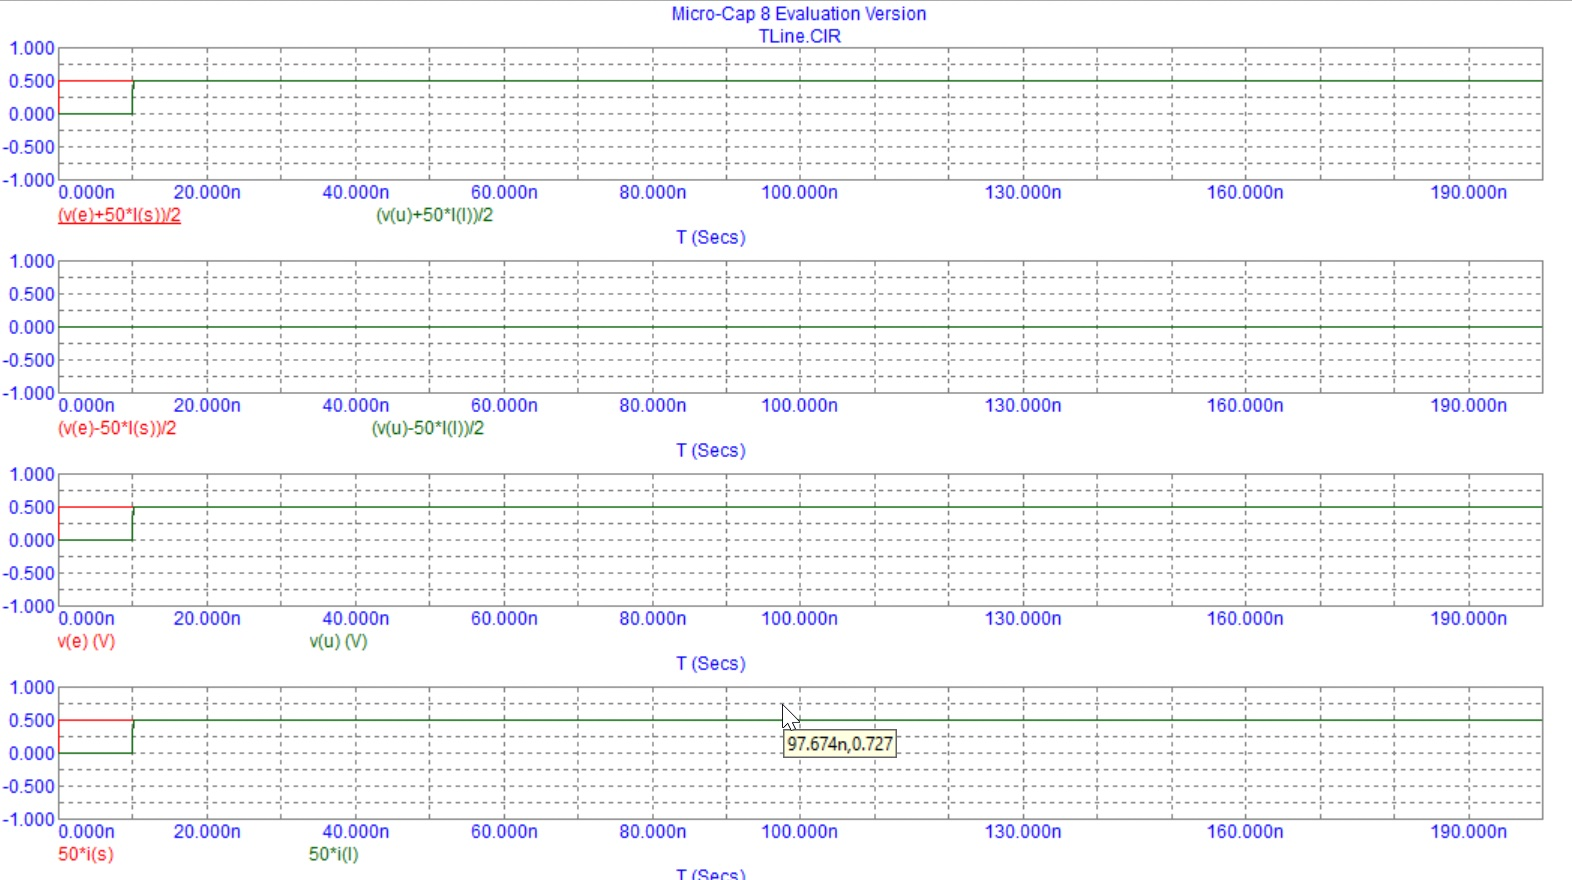
\includegraphics[width = 0.7\textwidth]{image_1}
	\caption{График для согласованной линии}
	\label{fig:image_1}
\end{figure}

\item\textbf{Рассогласованный источник}\\
	Рассогласовываем нагрузку источника: $R_s = \frac{\omega}{3};\ \rho_s = -\frac{1}{2}$. При этом мощность: 
$$
P\omega = v(u)i(l)\omega = 0.75 * 0.75 = 0.5625 = \frac{V^2}{4R_s}\omega(1-\rho_s^2)
$$
Теперь ставим: $R_s = 3\omega;\ \rho_s = \frac{1}{2}$. При этом мощность: 
$$
P\omega = v(u)i(l)\omega = 0.25 * 0.25 = 0.0625 = 			\frac{V^2}{4R_s}\omega(1-\rho_s^2)
$$
\begin{figure}[!h]
	\centering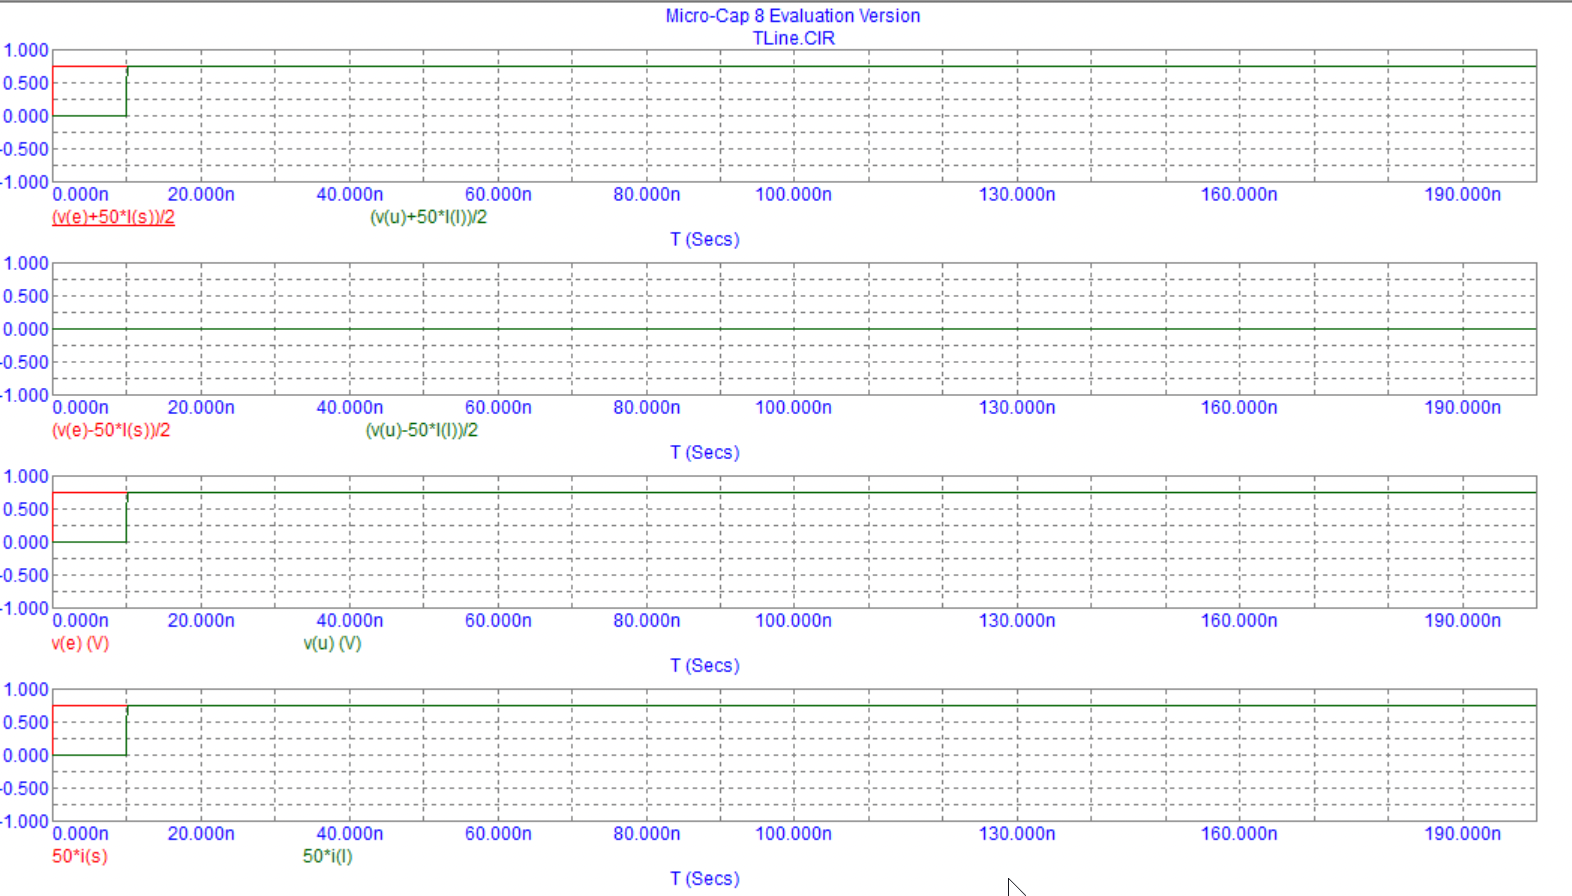
\includegraphics[width = 0.7\textwidth]{image_2}
	\caption{График для рассогласованного источника}
	\label{fig:image_2}
\end{figure}

\item\textbf{Рассогласованная нагрузка}\\
	Варьируем $R_l$. Наблюдаем, что установление происходит за две 'ступеньки': 1) волна прошла через длинный провод. 2) волна отразилась обратно. Таблица с измерениями:
\begin{table}[!h]
	\centering
	\begin{tabular}{|c|c|c|c|c|} \hline
		$R_l$ & $0$ & $\frac{\omega}{3}$ & $3\omega$ & $50k \simeq \infty$ \\ \hline 
		$\rho_l$ & $-1$ & $-\frac{1}{2}$ & $\frac{1}{2}$ & $1$ \\ \hline
		$(v + i\omega)/2, В$ & 0.5 & 0.5 & 0.5 & 0.5 \\ \hline
		$(v - i\omega)/2, В$ & -0.5 & -0.25 & 0.25 & 0.5 \\ \hline
		$v, В$ & 0 & 0.25 & 0.75 & 1 \\ \hline
		$i\omega, В$ & 1 & 0.75 & 0.25 & 0 \\ \hline
	\end{tabular}
\end{table}

\begin{figure}[!h]
	\centering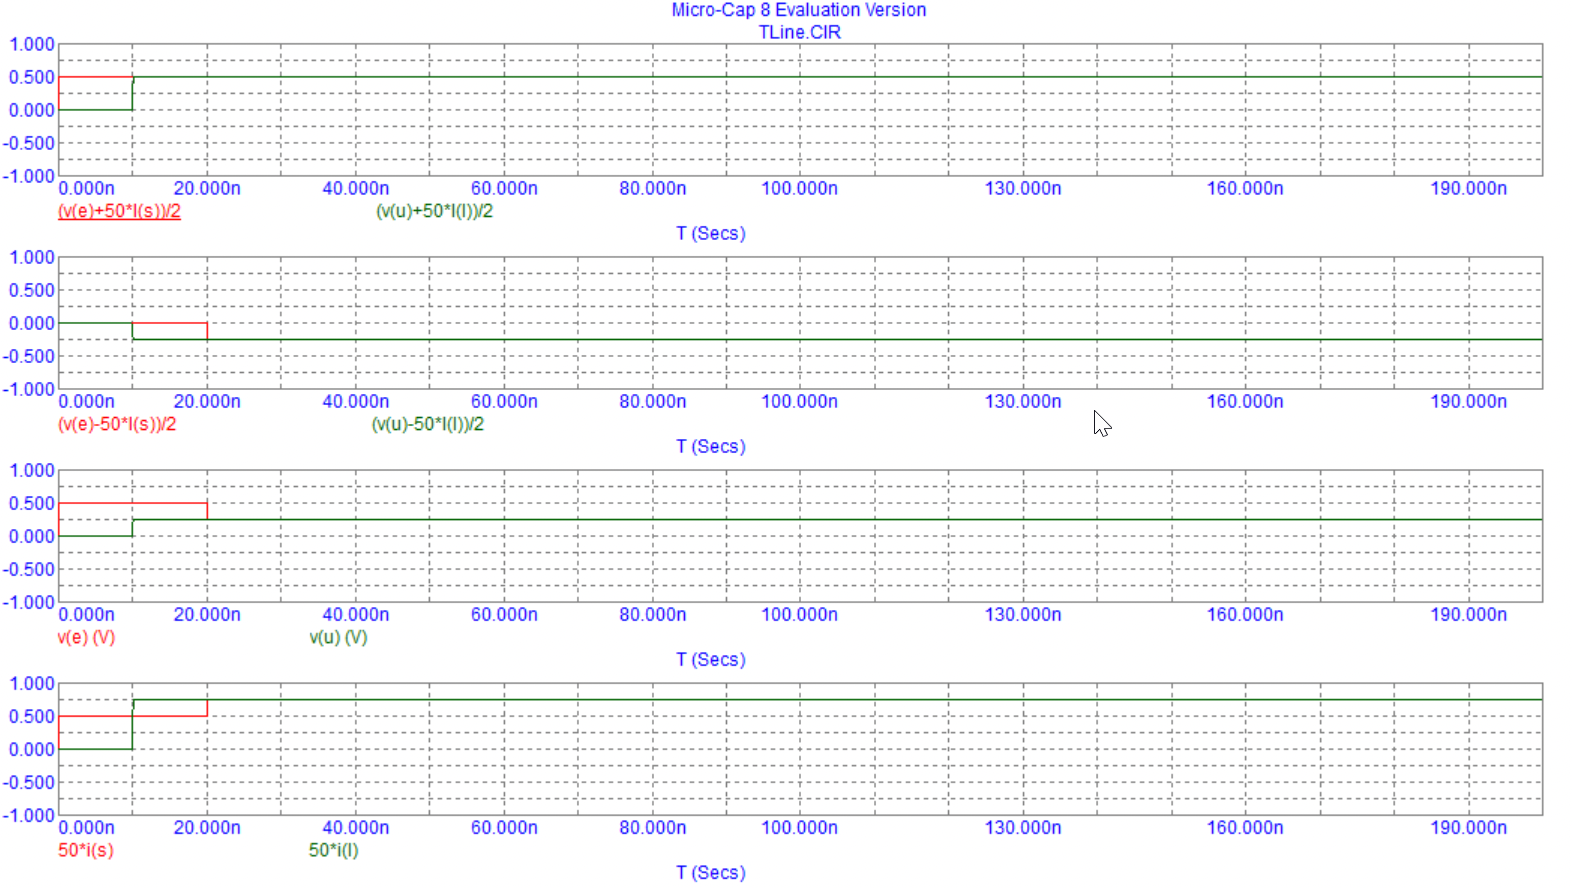
\includegraphics[width = 0.8\textwidth]{image_3}
	\caption{График при $R_l = \frac{\omega}{3}$}
	\label{fig:image_3}
\end{figure}

\newpage
\item\textbf{Рассогласованные источник и нагрузка}\\
Проведу наблюдения при разных значениях $R_l$ и $R_s$:
	\begin{table}[h!]
	\centering
	\begin{tabular}{|c|c|c|c|c|c|c|c|c|} \hline
		$R_s;\ R_l (Ом)$ & $50/3; 0$ & $50/3; 50k$ & $150; 0$ & $150; 50k$ & $0; 0$ & $0; 5$ & $0; 500$ & $0; 50k$ \\ \hline 
		$\rho_s\rho_l$ & $\frac{1}{2}$ & $-\frac{1}{2}$ & $-\frac{1}{2}$ & $\frac{1}{2}$ & $1$ & $-0.8$ & $0.8$ & $1$  \\ \hline
		$(v + i\omega)/2, В$ & 1.5 & 0.5 & 0.1667 & 0.5 & $\infty$ & 5 & 0.5556 & 1 или 0 \\ \hline
		$(v - i\omega)/2, В$ & -1.5 & 0.5 & -0.1667 & 0.5 & $-\infty$ & -4 & 0.4444 & 1 или 0\\ \hline
		$v, В$ & 0 & 1 & 0 & 1 & $1; 0$ & 1 & 1 & $1; 1 \pm 1$ \\ \hline
		$i\omega, В$ & 3 & 0 & 0.3333 & 0 & $\infty$ & 9 & 0.1111 & $\pm 1; 0$ \\ \hline
	\end{tabular}
\end{table}


\item\textbf{Ёмкостная наргузка}\\
По графикам переходного процесса найдем постоянную времени. За это время ток уменьшается до уровня $\frac{1}{e}$. Получаем $\tau \simeq 5\ нс$. Это значение согласуется с формулой $\tau = \omega C$.

При $R_s = 50$: $A = 0.5;\ B = 0.5;\ v = 1;\ i\omega = 0$. При $R_s = 50/3$ аналогично. \\

Отдельно рассмотрим случай $R_s = 0$. Дело в том, что графики трудно анализируемой формы, однако можно заметить, что они периодичны с периодом T = 60 нс. Установившихся значений определить нельзя, потому что они и не устанавливаются.

\begin{figure}[!h]
	\centering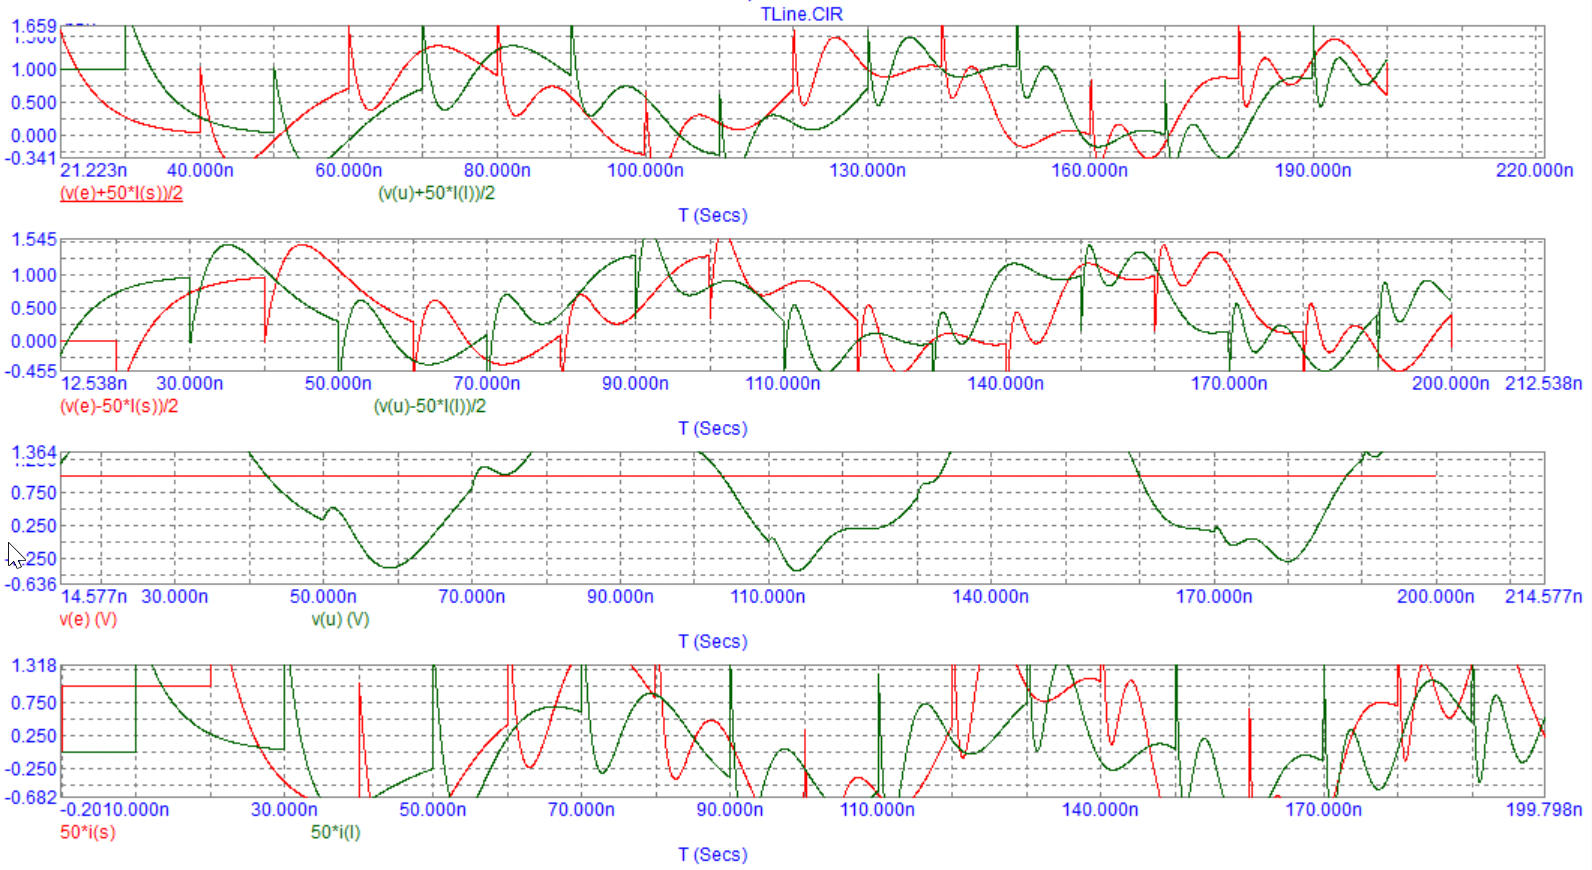
\includegraphics[width = \textwidth]{image_4}
	\caption{График при $R_s = 0$}
	\label{fig:image_4}
\end{figure}

\end{enumerate}
\end{document}